\section{选择题}
\begin{ti}
	设有下列命题
	\begin{enumerate}
		\item 数列 $\{ x_n \}$ 收敛(即 $\exists$ 极限 $\lim_{n \to \infty} x_n$),则 $x_n$ 有界。
		\item 数列极限 $\lim_{n \to \infty} x_n = a \Leftrightarrow \lim_{n \to \infty} x_{n+l} = a$。其中 $l$ 为某个确定的正整数。
		\item 数列 $\lim_{n \to \infty} x_n = a \Leftrightarrow \lim_{n \to \infty} x_{2n-1} = \lim_{n \to \infty} x_{2n} = a$。
		\item 数列极限 $\lim_{n \to \infty} x_n \exists \Leftrightarrow \lim_{n \to \infty} \frac{x_{n+1}}{x_n} = 1$。
	\end{enumerate}
	则以上命题中正确的个数是
	\begin{tasks}(4)
		\task 1。
		\task 2。
		\task 3。
		\task 4。
	\end{tasks}
\end{ti}

\begin{ti}
	设 $x_n \leq z_n \leq y_n$,且 $\lim_{n \to \infty} (y_n - x_n) = 0$,则 $\lim_{n \to \infty} z_n$
	\begin{tasks}(2)
		\task 存在且等于零。
		\task 存在但不一定等于零。
		\task 不一定存在。
		\task 一定不存在。
	\end{tasks}
\end{ti}

\begin{ti}
	有以下命题:设 $\lim_{x \to a} f(x) = A$, $\lim_{x \to a} g(x)$ 不 $\exists$, $\lim_{x \to a} h(x)$ 不 $\exists$,
	\begin{enumerate}
		\item $\lim_{x \to a} (f(x) \cdot g(x))$ 不 $\exists$。
		\item $\lim_{x \to a} (g(x) + h(x))$ 不 $\exists$。
		\item $\lim_{x \to a} (h(x) \cdot g(x))$ 不 $\exists$。
		\item $\lim_{x \to a} (g(x) + f(x))$ 不 $\exists$。
	\end{enumerate}
	则以上命题中正确的个数是
	\begin{tasks}(4)
		\task 0。
		\task 1。
		\task 2。
		\task 3。
	\end{tasks}
\end{ti}

\begin{ti}
	下列叙述正确的是
	\begin{tasks}
		\task 如果 $f(x)$ 在 $x_0$ 的任意空心邻域内无界,则 $\lim_{x \to x_0} f(x) = \infty$。
		\task 如果 $\lim_{x \to x_0} f(x) = \infty$,则 $f(x)$ 在 $x_0$ 的任意空心邻域内无界。
		\task $\lim_{x \to x_0} f(x)$ 不存在,则 $\lim_{x \to x_0} f(x) = \infty$。
		\task 如果 $\lim_{x \to x_0} f(x) = 0$,则 $\lim_{x \to x_0} \frac{1}{f(x)} = \infty$。
	\end{tasks}
\end{ti}

\begin{ti}
	下列命题中正确的是
	\begin{tasks}
		\task 若 $\lim_{x \to x_0} f(x) \geq \lim_{x \to x_0} g(x) \Rightarrow \exists \delta > 0$,当 $0 < |x-x_0| < \delta$ 时 $f(x) \geq g(x)$。\xeCJKnobreak
		\task 若 $\exists \delta > 0$ 使得当 $0 < |x-x_0| < \delta$ 时有 $f(x) > g(x)$ 且 $\lim_{x \to x_0} f(x) = A_0$, $\lim_{x \to x_0} g(x) = B_0$ 均 $\exists$,则 $A_0 > B_0$。
		\task 若 $\exists \delta > 0$,当 $0 < |x-x_0| < \delta$ 时 $f(x) > g(x) \Rightarrow \lim_{x \to x_0} f(x) \geq \lim_{x \to x_0} g(x)$。\xeCJKnobreak
		\task 若 $\lim_{x \to x_0} f(x) \geq \lim_{x \to x_0} g(x) \Rightarrow \exists \delta > 0$,当 $0 < |x-x_0| < \delta$ 时有 $f(x) > g(x)$。
	\end{tasks}
\end{ti}

\begin{ti}
	$\lim_{n \to \infty} \sin^2\bigl( \uppi \sqrt{n^2+n} \bigr) = $
	\begin{tasks}(4)
		\task $1$。
		\task $\frac{3}{4}$。
		\task $\frac{1}{2}$。
		\task $\frac{1}{4}$。
	\end{tasks}
\end{ti}

\begin{ti}
	当 $n \to \infty$ 时,$\ee - \biggl(1 + \frac{1}{n}\biggr)^n$ 与 $An^{-p}$ 为等价无穷小,则
	\begin{tasks}(2)
		\task $A = \frac{\ee}{3}$, $p = 1$。
		\task $A = \frac{\ee}{2}$, $p = 1$。
		\task $A = \frac{\ee}{3}$, $p = 2$。
		\task $A = \frac{\ee}{2}$, $p = 2$。
	\end{tasks}
\end{ti}

\begin{ti}
	$\lim_{n \to \infty} \biggl( \frac{1}{n^2+n+1} + \frac{2}{n^2+n+2} + \cdots + \frac{n}{n^2+n+n} \biggr) = $
	\begin{tasks}(4)
		\task $3$。
		\task $2$。
		\task $\frac{2}{3}$。
		\task $\frac{1}{2}$。
	\end{tasks}
\end{ti}

\begin{ti}
	$f(x) = \frac{\sin \uppi x}{x-1} \ee^{\frac{1}{(x-1)^3}}$,则当 $x \to 1$ 时有
	\begin{tasks}
		\task $\lim_{x \to 1} f(x) = - \uppi$。
		\task $\lim_{x \to 1} f(x) = 0$。
		\task $\lim_{x \to 1} f(x) = \infty$。
		\task $\lim_{x \to 1} f(x)$ 不存在,且 $\lim_{x \to 1} f(x) \ne \infty$。
	\end{tasks}
\end{ti}

\begin{ti}
	$I = \lim_{x \to 0} \frac{\cos( x\ee^x ) - \ee^{-\frac{x^2}{2} \ee^{2x}}}{x^4} = $
	\begin{tasks}(4)
		\task $0$。
		\task $-\frac{1}{6}$。
		\task $-\frac{1}{8}$。
		\task $-\frac{1}{12}$。
	\end{tasks}
\end{ti}

\begin{ti}
	$\lim_{x \to \infty} \biggl( \cos\frac{1}{x} \biggr)^{x^2} = $
	\begin{tasks}(4)
		\task 1。
		\task $\ee$。
		\task $\ee^{\frac{1}{2}}$。
		\task $\ee^{-\frac{1}{2}}$。
	\end{tasks}
\end{ti}

\begin{ti}
	$\lim_{x \to 0} \frac{\cos(\sin x) - \cos x}{(1 - \cos x) \sin^2x} = $
	\begin{tasks}(4)
		\task $1$。
		\task $\frac{1}{2}$。
		\task $\frac{1}{3}$。
		\task $0$。
	\end{tasks}
\end{ti}

\begin{ti}
	$\lim_{x \to +\infty} \frac{\bigl( 1 + \frac{1}{x} \bigr)^{x^2}}{\ee^x} = $
	\begin{tasks}(4)
		\task $0$。
		\task $\ee^{-\frac{1}{4}}$。
		\task $\ee^{-\frac{1}{3}}$。
		\task $\ee^{-\frac{1}{2}}$。
	\end{tasks}
\end{ti}

\begin{ti}
	已知 $I = \lim_{x \to 0} \frac{ax^2 + bx + 1 - \ee^{x^2-2x}}{x^2} = 2$,则
	\begin{tasks}(2)
		\task $a = 5$, $b = -2$。
		\task $a = -2$, $b = 5$。
		\task $a = 2$, $b = 0$。
		\task $a = 3$, $b = -3$。
	\end{tasks}
\end{ti}

\begin{ti}
	设 $\lim_{x \to 0} \frac{\sin 6x - (\sin x) f(x)}{x^3} = 0$,则 $\lim_{x \to 0} \frac{6-f(x)}{x^2} = $
	\begin{tasks}(4)
		\task $0$。
		\task $35$。
		\task $36$。
		\task $\infty$。
	\end{tasks}
\end{ti}

\begin{ti}
	下列各题计算过程中正确无误的是
	\begin{tasks}
		\task 数列极限 $\lim_{n \to \infty} \frac{\ln n}{n} = \lim_{n \to \infty} \frac{(\ln n)'}{n'} = \lim_{n \to \infty} \frac{1}{n} = 0$。
		\task $\lim_{x \to 1} \frac{\sin \uppi x}{3x^2 - 2x - 1} = \lim_{x \to 1} \frac{\uppi \cos \uppi x}{6x - 2} = \lim_{x \to 1} \frac{-\uppi^2 \sin \uppi x}{6} = 0$。
		\task $\lim_{x \to 0} \frac{x^2 \sin \frac{1}{x}}{\sin x} = \lim_{x \to 0} \frac{2x \sin \frac{1}{x} - \cos \frac{1}{x}}{\cos x}$ 不存在。
		\task $\lim_{x \to 0} \frac{x + \sin x}{x - \sin x} = \lim_{x \to 0} \frac{1 + \cos x}{1 - \cos x} = \infty$。
	\end{tasks}
\end{ti}

\begin{ti}
	当 $n \to \infty$ 时,数列 $\biggl( 1 + \frac{1}{n} \biggr)^n - \ee$ 是 $\frac1n$ 的
	\begin{tasks}(2)
		\task 高阶无穷小。
		\task 低阶无穷小。
		\task 等价无穷小。
		\task 同阶但非等价无穷小。
	\end{tasks}
\end{ti}

\begin{ti}
	当 $x \to 0$ 时下列无穷小中阶数最高的是
	\begin{tasks}(2)
		\task $(1 + x)^{x^2} - 1$。
		\task $\ee^{x^4-2x} - 1$。
		\task $\int_0^{x^2} \sin t^2 \dd{t}$。
		\task $\sqrt{1+2x} - \sqrt[3]{1+3x}$。
	\end{tasks}
\end{ti}

\begin{ti}
	设 $x \to a$ 时 $f(x)$ 与 $g(x)$ 分别是 $x-a$ 的 $n$ 阶与 $m$ 阶无穷小,则下列命题
	\begin{enumerate}
		\item $f(x) g(x)$ 是 $x-a$ 的 $n+m$ 阶无穷小。
		\item 若 $n > m$,则 $\frac{f(x)}{g(x)}$ 是 $x-a$ 的 $n-m$ 阶无穷小。
		\item 若 $n \leq m$,则 $f(x) + g(x)$ 是 $x-a$ 的 $n$ 阶无穷小。
		\item 若 $f(x)$ 连续,则 $\int_a^x f(t) \dd{t}$ 是 $x-a$ 的 $n+1$ 阶无穷小。
	\end{enumerate}
	中,正确的个数是
	\begin{tasks}(4)
		\task 1。
		\task 2。
		\task 3。
		\task 4。
	\end{tasks}
\end{ti}

\begin{ti}
	设 $f(x) = \int_0^x t \ee^{\sin t} \dd{t}$,则当 $x \to 0$ 时,$f(x)$ 为无穷小 $x$ 的阶为
	\begin{tasks}(4)
		\task 1 阶。
		\task 2 阶。
		\task 3 阶。
		\task 4 阶。
	\end{tasks}
\end{ti}

\begin{ti}
	以下函数 $f(g(x))$ 以 $x=0$ 为第二类间断点的是
	\begin{tasks}
		\task $f(u) = \ln(1+u^2)$, $g(u) = \begin{cases}
			\sin^2x + (x+1)^2, & x \leq 0, \\
			x^2+1, & x > 0.
		\end{cases}$
		\task $f(u) = \begin{cases}
			1-u, & u \leq 0 \\
			u^2 + 1, & u > 0
		\end{cases}$, $g(x) = 2\cos x-1$。
		\task $f(u) = \begin{cases}
			\frac{\ln(1-u^2)}{u} \sin\frac{1}{u}, & u < 0 \\
			1 - \cos\sqrt{u}, & u \geq 0
		\end{cases}$, $g(x) = \begin{cases}
			x, & x < 0, \\
			x + \frac{\uppi^2}{4}, & x \geq 0.
		\end{cases}$
		\task $f(u) = \ee^{u^2} + 1$, $g(x) = \begin{cases}
			\frac{1}{x}, & x < 0, \\
			0, & x = 0, \\
			\sin\frac{1}{x}, & x > 0.
		\end{cases}$
	\end{tasks}
\end{ti}

\begin{ti}
	设 $f(x) = \frac{1}{\arctan\frac{x-1}{x}}$ 则
	\begin{tasks}
		\task $x=0$ 与 $x=1$ 都是 $f(x)$ 的第一类间断点。
		\task $x=0$ 与 $x=1$ 都是 $f(x)$ 的第二类间断点。
		\task $x=0$ 是 $f(x)$ 的第一类间断点,$x=1$ 是 $f(x)$ 的第二类间断点。
		\task $x=0$ 是 $f(x)$ 的第二类间断点,$x=1$ 是 $f(x)$ 的第一类间断点。
	\end{tasks}
\end{ti}

\begin{ti}
	设 $f(x)$ 在点 $x_0$ 的某邻域内有定义,且 $f(x)$ 在 $x_0$ 间断,则在点 $x_0$ 处必定间断的函数是
	\begin{tasks}(4)
		\task $f(x) \sin x$。
		\task $f(x) + \sin x$。
		\task $f^2(x)$。
		\task $|f(x)|$。
	\end{tasks}
\end{ti}

\begin{ti}
	“$f(x)$ 在 $x_0$ 点连续”是 $|f(x)|$ 在 $x_0$ 点连续的
	\begin{tasks}(2)
		\task 充分条件,但不是必要条件。
		\task 必要条件,但不是充分条件。
		\task 充分必要条件。
		\task 既不是充分,也不是必要条件.
	\end{tasks}
\end{ti}

\begin{ti}
	设 $f(x)$ 在 $[a,+\infty)$ 连续,则“$\exists x_n \in [a,+\infty)$ 有 $\lim_{n \to \infty}x_n = +\infty$ 且 $\lim_{n \to \infty}f(x_n) = \infty$”是 $f(x)$ 在 $[a,+\infty)$ 无界的
	\begin{tasks}(2)
		\task 充分非必要条件。
		\task 必要非充分条件。
		\task 充要条件。
		\task 既非充分又非必要条件。
	\end{tasks}
\end{ti}

\begin{ti}
	设 $f(x) = \begin{cases}
		\frac{1-\cos x^2}{x^3}, & x > 0 \\
		g(x) \arcsin^2x, & x \leq 0
	\end{cases}$,其中 $g(x)$ 是有界函数,则 $f(x)$ 在 $x=0$ 处
	\begin{tasks}(2)
		\task 极限不存在。
		\task 极限存在,但不连续。
		\task 连续,但不可导。
		\task 可导。
	\end{tasks}
\end{ti}

\begin{ti}
	设 $f(x) = \begin{cases}
		\ee^{\frac{1}{x^2-1}}, & |x|<1 \\
		x^4 - bx^2 + c, & |x| \geq 1
	\end{cases}$ 可导,则 $(b,c) = $
	\begin{tasks}(4)
		\task $(2,1)$。
		\task $(1,0)$。
		\task $\biggl(\frac{1}{2},-\frac{1}{2}\biggr)$。
		\task $(3,2)$。
	\end{tasks}
\end{ti}

\begin{ti}
	下列函数 $f(x)$ 中,导函数 $f'(x)$ 在 $x=0$ 处不连续的是
	\begin{tasks}(2)
		\task $f(x) = \begin{cases}
			x^{\frac43} \sin \frac{1}{x}, & x \ne 0 \\
			0, & x = 0
		\end{cases}$。
		\task $f(x) = \begin{cases}
			\frac{\sin x}{x}, & x \ne 0 \\
			1, & x = 0
		\end{cases}$。
		\task $f(x) = \begin{cases}
			\frac{\ee^x-1}{x}, & x \ne 0 \\
			1, & x = 0
		\end{cases}$。
		\task $f(x) = \begin{cases}
			\frac{\ln(1+x)}{x}, & x \ne 0 \\
			1, & x = 0
		\end{cases}$。
	\end{tasks}
\end{ti}

\begin{ti}
	设 $f(0) = 0$,则 $\lim_{x \to 0} \frac{f\bigl(x^2\bigr)}{x^2}$ 存在是 $f(x)$ 在 $x=0$ 可导的
	\begin{tasks}(2)
		\task 充分非必要条件。
		\task 必要非充分条件。
		\task 充分必要条件。
		\task 既非充分又非必要条件。
	\end{tasks}
\end{ti}

\begin{ti}
	设 $f(x)$ 是以 $3$ 为周期的可导函数且 $f'(4) = 1$,则
	\[\lim_{h \to 0} \frac{f(1+h) - f(1-3\tan h)}{h}\]
	等于
	\begin{tasks}(4)
		\task $5$。
		\task $3$。
		\task $4$。
		\task $7$。
	\end{tasks}
\end{ti}

\begin{ti}
  设函数 $g(x)$ 在 $x=a$ 点处连续,$f(x) = |x-a| g(x)$ 在 $x=a$ 点处可导,则 $g(a)$ 满足
  \begin{tasks}(4)
    \task $g(a) = a$。
    \task $g(a) \ne a$。
    \task $g(a) = 0$。
    \task $g(a) \ne 0$。
  \end{tasks}
\end{ti}

\begin{ti}
	设 $f(x) = |x| \sin^2x$,则使 $f^{(n)}(0)$ 存在的最高阶数 $n = $
	\begin{tasks}(4)
		\task $0$。
		\task $1$。
		\task $2$。
		\task $3$。
	\end{tasks}
\end{ti}

\begin{ti}
	设 $f(x)$ 在点 $x=a$ 处可导,则函数 $|f(x)|$ 在点 $x=a$ 处不可导的充分必要条件是
	\begin{tasks}(2)
		\task $f(a) = 0$,且 $f'(a) = 0$。
		\task $f(a) = 0$,且 $f'(a) \ne 0$。
		\task $f(a) > 0$,且 $f'(a) > 0$。
		\task $f(a) < 0$,且 $f'(a) < 0$。
	\end{tasks}
\end{ti}

\begin{ti}
	设 $\lim_{x \to x_0^+} f'(x) = \lim_{x \to x_0^-} f'(x) = a$,则
	\begin{tasks}
		\task $f(x)$ 在 $x=x_0$ 处必可导且 $f'(x_0) = a$。
		\task $f(x)$ 在 $x=x_0$ 处必连续,但未必可导。
		\task $f(x)$ 在 $x=x_0$ 处必有极限但未必连续。
		\task 以上结论都不对。
	\end{tasks}
\end{ti}

\begin{ti}
	设 $f(x)$ 为连续函数,$g(x) = \int_{-x}^0 tf(x+t) \dd{t}$,则 $g'(x) = $
	\begin{tasks}(2)
		\task $-\int_0^x f(u) \dd{u}$。
		\task $\int_0^x f(u) \dd{u}$。
		\task $-\int_0^{-x} f(u) \dd{u}$。
		\task $\int_0^{-x} f(u) \dd{u}$。
	\end{tasks}
\end{ti}

\begin{ti}
	设直线 $y=ax+b$ 同时与曲线 $y=x^2$ 及 $y = \frac{1}{x}$ 相切,则常数 $a$, $b$ 为
	\begin{tasks}(2)
		\task $a=-4$, $b=-4$。
		\task $a=-3$, $b=-4$。
		\task $a=-4$, $b=-3$。
		\task $a=-3$, $b=-3$。
	\end{tasks}
\end{ti}

\begin{ti}
	\parbox[c]{0.6\textwidth}{%
	在曲线 $y = \frac{1}{x}$ ($0 < x < +\infty$) 上任一点 $P(x,y)$ 处作切线,该切线分别交 $x$ 轴与 $y$ 轴于 $A$ 和 $B$(如图所示),则
	\begin{tasks}
		\task $\overline{PA} < \overline{PB}$。
		\task $\overline{PA} = \overline{PB}$。
		\task $\overline{PA} > \overline{PB}$。
		\task $\overline{PA}$, $\overline{PB}$ 的大小关系与 $P$ 的位置有关。
	\end{tasks}
	}%
	\begin{varwidth}[c]{\textwidth}
		\vspace{0pt}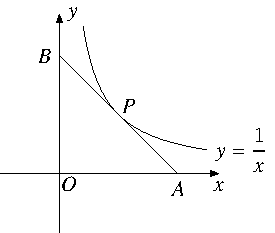
\includegraphics{figure/fig157.pdf}
	\end{varwidth}
\end{ti}

\begin{ti}
	设 $f(x)$ 在 $x_0$ 可导,且 $f'(x_0)>0$,则 $\exists \delta > 0$,使得
	\begin{tasks}
		\task $f(x)$ 在 $(x_0-\delta,x_0+\delta)$ 单调上升。
		\task $f(x)>f(x_0)$, $x \in (x_0-\delta,x_0+\delta)$, $x \ne x_0$。
		\task $f(x)>f(x_0)$, $x \in (x_0,x_0+\delta)$。
		\task $f(x)<f(x_0)$, $x \in (x_0,x_0+\delta)$。
	\end{tasks}
\end{ti}

\begin{ti}
	设 $f(x)$ 对一切 $x \in (-\infty,+\infty)$ 满足方程 $(x-1) f''(x) + 2(x-1) [f'(x)]^3 = 1 - \ee^{1-x}$,且 $f(x)$ 在 $x=a$ ($a \ne 1$) 处 $f'(a) = 0$,则 $x = a$
	\begin{tasks}(2)
		\task 是 $f(x)$ 的极小值点。
		\task 是 $f(x)$ 的极大值点。
		\task 不是 $f(x)$ 的极值点。
		\task 是 $f(x)$ 的拐点。
	\end{tasks}
\end{ti}

\begin{ti}
	设 $f(x)$ 具有二阶连续导数,且 $f'(1)=0$, $\lim_{x \to 1} \frac{f''(x)}{(x-1)^2} = \frac{1}{2}$,则
	\begin{tasks}
		\task $f(1)$ 是 $f(x)$ 的极大值。
		\task $f(1)$ 是 $f(x)$ 的极小值。
		\task $(1,f(1))$ 是曲线 $f(x)$ 的拐点坐标。
		\task $f(1)$ 不是 $f(x)$ 的极值,$(1,f(1))$ 也不是曲线 $f(x)$ 的拐点坐标。
	\end{tasks}
\end{ti}

\begin{ti}
	设 $f(x) = \begin{cases}
		2 - \cos x, & x \leq 0 \\
		\sqrt{x} + 1, & x > 0
	\end{cases}$,则
	\begin{tasks}
		\task $x=0$ 是 $f(x)$ 的极值点,但 $(0,1)$ 不是曲线 $y=f(x)$ 的拐点。
		\task $x=0$ 不是 $f(x)$ 的极值点,但 $(0,1)$ 是曲线 $y=f(x)$ 的拐点。
		\task $x=0$ 是 $f(x)$ 的极值点,且 $(0,1)$ 是曲线 $y=f(x)$ 的拐点。
		\task $x=0$ 不是 $f(x)$ 的极值点,$(0,1)$ 也不是曲线 $y=f(x)$ 的拐点。
	\end{tasks}
\end{ti}

\begin{ti}
	设函数 $f(x)$ 在 $(-\infty,+\infty)$ 上有定义,则下述命题中正确的是
	\begin{tasks}
		\task 若 $f(x)$ 在 $(-\infty,+\infty)$ 上可导且单调增加,则对一切 $x \in (-\infty,+\infty)$,都有 $f'(x) > 0$。
		\task 若 $f(x)$ 在点 $x_0$ 处取得极值,则 $f'(x_0) = 0$。
		\task 若 $f''(x_0) = 0$,则 $(x_0,f(x_0))$ 是曲线 $y=f(x)$ 的拐点坐标。
		\task 若 $f'(x_0) = 0$, $f''(x_0) = 0$, $f'''(x_0) \ne 0$,则 $x_0$ 一定不是 $f(x)$ 的极值点。
	\end{tasks}
\end{ti}

\begin{ti}
	设 $f(x)$ 在 $[a,b]$ 可导,$f(a) = \max_{[a,b]} f(x)$,则
	\begin{tasks}(2)
		\task $f_{+}'(a) = 0$。
		\task $f_{+}'(a) \geq 0$。
		\task $f_{+}'(a) < 0$。
		\task $f_{+}'(a) \leq 0$。
	\end{tasks}
\end{ti}

\begin{ti}
	数列 $1$, $\sqrt{2}$, $\sqrt[3]{3}$, $\cdots$, $\sqrt[n]{n}$, $\cdots$ 的最大项为
	\begin{tasks}(4)
		\task $\sqrt{2}$。
		\task $\sqrt[3]{3}$。
		\task $\sqrt[4]{4}$。
		\task $\sqrt[5]{5}$。
	\end{tasks}
\end{ti}

\begin{ti}
	设 $f(x) = ax^3 - 6ax^2 + b$ 在区间 $[-1,2]$ 上的最大值是 $3$,最小值是 $-29$,且 $a>0$,则
	\begin{tasks}(2)
		\task $a=2$, $b=-29$。
		\task $a=3$, $b=2$。
		\task $a=2$, $b=3$。
		\task 以上都不对。
	\end{tasks}
\end{ti}

\begin{ti}
	曲线 $\begin{cases}
		x = a(t - \sin t), \\
		y = a(1 - \cos t),
	\end{cases}$ ($a > 0$) 在参数 $t = \frac{\uppi}{2}$ 对应的点处的曲率为
	\begin{tasks}(4)
		\task $\frac{2\sqrt{2}}{a}$。
		\task $\frac{\sqrt{2}}{a}$。
		\task $\frac{1}{\sqrt{2}a}$。
		\task $\frac{1}{2\sqrt{2}a}$。
	\end{tasks}
\end{ti}

\begin{ti}
	以下四个命题中,正确的是
	\begin{tasks}
		\task 若 $f'(x)$ 在 $(a,b)$ 内连续,则 $f(x)$ 在 $(a,b)$ 内有界。
		\task 若 $f(x)$ 在 $(a,b)$ 内连续,则 $f(x)$ 在 $(a,b)$ 内有界。
		\task 若 $f'(x)$ 在 $(a,b)$ 内有界,则 $f(x)$ 在 $(a,b)$ 内有界。
		\task 若 $f(x)$ 在 $(a,b)$ 内有界,则 $f'(x)$ 在 $(a,b)$ 内有界。
	\end{tasks}
\end{ti}

\begin{ti}
	设 $f(x)$ 在 $(a,+\infty)$ 可导,则 $f'(x)$ 在 $(a,+\infty)$ 有界是 $f(x)$ 在 $(a,+\infty)$ 有界的
	\begin{tasks}(2)
		\task 必要非充分条件。
		\task 充分非必要条件。
		\task 充分且必要条件。
		\task 既非充分也非必要条件。
	\end{tasks}
\end{ti}

\begin{ti}
	\parbox[t]{0.7\textwidth}{\vspace{0pt}%
	函数 $y=f(x)$ 在 $(-\infty,+\infty)$ 连续,其二阶导函数的图形如图所示,则 $y=f(x)$ 的拐点的个数是
	\begin{tasks}(4)
		\task $1$。
		\task $2$。
		\task $3$。
		\task $4$。
	\end{tasks}
	}%
	\begin{varwidth}[t]{\textwidth}
		\vspace{0pt}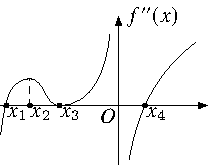
\includegraphics{figure/fig169.pdf}
	\end{varwidth}
\end{ti}

\begin{ti}
	\parbox[t]{0.58\textwidth}{\vspace{0pt}%
	设 $[0,+\infty)$ 区间上 $y=f(x)$ 的导函数的图形如下图所示,则 $y=f(x)$ 的拐点的个数是
	\begin{tasks}(4)
		\task $1$。
		\task $2$。
		\task $3$。
		\task $4$。
	\end{tasks}
	}%
	\begin{varwidth}[t]{\textwidth}
		\vspace{0pt}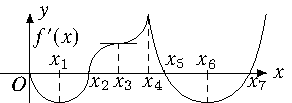
\includegraphics{figure/fig170.pdf}
	\end{varwidth}
\end{ti}

\begin{ti}
	设曲线 $y = \sqrt[3]{x-4}$,则
	\begin{tasks}
		\task 曲线的凸区间为 $(-\infty,4)$,凹区间为 $(4,+\infty)$,拐点为 $(4,0)$。
		\task 曲线的凹区间为 $(-\infty,4)$,凸区间为 $(4,+\infty)$,拐点为 $(4,0)$。
		\task 曲线的凸区间为 $(-\infty,4)$,凹区间为 $(4,+\infty)$,无拐点。
		\task 曲线的凹区间为 $(-\infty,4)$,凸区间为 $(4,+\infty)$,无拐点。
	\end{tasks}
\end{ti}

\begin{ti}
	函数 $f(x) = 3 \arccos x - \arccos (3x-4x^3)$ 在 $\biggl[ -\frac{1}{2},\frac{1}{2} \biggr]$
	\begin{tasks}(2)
		\task 单调上升。
		\task 单调下降。
		\task 为常数。
		\task 有两个单调性区间。
	\end{tasks}
\end{ti}

\begin{ti}
	设 $f(x)$ 在 $(1-\delta,1+\delta)$ 内存在导数,$f'(x)$ 单调减少,且 $f(1) = f'(1) = 1$,则
	\begin{tasks}
		\task 在 $(1-\delta,1)$ 和 $(1,1+\delta)$ 内均有 $f(x) < x$。
		\task 在 $(1-\delta,1)$ 和 $(1,1+\delta)$ 内均有 $f(x) > x$。
		\task 在 $(1-\delta,1)$ 内有 $f(x) < x$,在 $(1,1+\delta)$ 内有 $f(x) > x$。
		\task 在 $(1-\delta,1)$ 内有 $f(x) > x$,在 $(1,1+\delta)$ 内有 $f(x) < x$。
	\end{tasks}
\end{ti}

\begin{ti}
	曲线 $y = \frac{x^2+1}{\sqrt{x^2-1}}$
	\begin{tasks}(2)
		\task 既有垂直又有水平与斜渐近线。\xeCJKnobreak
		\task 仅有垂直渐近线。
		\task 只有垂直与水平渐近线。
		\task 只有垂直与斜渐近线。
	\end{tasks}
\end{ti}

\begin{ti}
	函数 $f(x) = \cos x + x \sin x$ 在 $(-2\uppi,2\uppi)$ 内的零点个数为
	\begin{tasks}(4)
		\task $1$ 个。
		\task $2$ 个。
		\task $3$ 个。
		\task $4$ 个。
	\end{tasks}
\end{ti}

\begin{ti}
	设 $F(x)$ 是 $f(x)$ 在 $(a,b)$ 上的一个原函数,则 $f(x) + F(x)$ 在 $(a,b)$ 上
	\begin{tasks}(2)
		\task 可导。
		\task 连续。
		\task 存在原函数。
		\task 是初等函数。
	\end{tasks}
\end{ti}

\begin{ti}
	设 $f(x) = \begin{cases}
		\sin \frac{1}{x}, & x \ne 0 \\
		1, & x = 0
	\end{cases}$, $F(x) = \int_{-1}^x f(t) \dd{t}$,则 $F(x)$
	\begin{tasks}(2)
		\task 在 $(-1,1)$ 为无界函数。
		\task 在 $(-1,1)$ 为连续有界函数。
		\task 在 $(-1,1)$ 有间断点 $x=0$。
		\task 在 $[-1,1]$ 不可积。
	\end{tasks}
\end{ti}

\begin{ti}
	设 $f(x)$ 一阶可导,$f(x) > 0$, $f'(x) > 0$,则当 $\Delta x > 0$ 时
	\begin{tasks}(2)
		\task $\int_x^{x+\Delta x} f(t) \dd{t} > f(x) \Delta x > 0$。
		\task $\int_x^{x+\Delta x} f(t) \dd{t} < f(x) \Delta x < 0$。
		\task $f(x) \Delta x > \int_x^{x+\Delta x} f(t) \dd{t} > 0$。
		\task $f(x) \Delta x < \int_x^{x+\Delta x} f(t) \dd{t} < 0$。
	\end{tasks}
\end{ti}

\begin{ti}
	考察下列叙述:
	\begin{enumerate}
		\item 设 $f^2(x)$ 在 $x=x_0$ 连续,则 $f(x)$ 在 $x=x_0$ 连续。\label{179-1}
		\item 设 $f(x)$ 在 $x=x_0$ 连续,则 $|f(x)|$ 在 $x=x_0$ 连续。\label{179-2}
		\item 设 $|f(x)|$ 在 $[a,b]$ 可积,则 $f(x)$ 在 $[a,b]$ 可积。\label{179-3}
		\item 设 $f(x)$ 在 $[a,b]$ 有界,只有有限个间断点,则 $|f(x)|$ 在 $[a,b]$ 可积,即在 $[a,b]$ 存在定积分。\label{179-4}
	\end{enumerate}
	我们可知
	\begin{tasks}(2)
		\task 只有 \eqref{179-1}, \eqref{179-2} 正确。
		\task 只有 \eqref{179-2}, \eqref{179-3} 正确。
		\task 只有 \eqref{179-2}, \eqref{179-4} 正确。
		\task 只有 \eqref{179-3}, \eqref{179-4} 正确。
	\end{tasks}
\end{ti}

\begin{ti}
	下列函数在指定区间上不存在定积分的是
	\begin{tasks}
		\task $f(x) = \begin{cases}
			\sin\frac{1}{x}, & x \ne 0 \\
			1, & x = 0
		\end{cases}$, $x \in [-1,1]$。
		\task $f(x) = \sgn x = \begin{cases}
			1, & x > 0 \\
			0, & x = 0 \\
			-1, & x < 0
		\end{cases}$, $x \in [a,b]$。
		\task $f(x) = \begin{cases}
			\tan x, & x \in \biggl( -\frac{\uppi}{2},\frac{\uppi}{2} \biggr) \\
			0, & x = \pm \frac{\uppi}{2}
		\end{cases}$, $x \in \biggl[ -\frac{\uppi}{2},\frac{\uppi}{2} \biggr]$。
		\task $f(x) = \begin{cases}
			\frac{\sin x}{x}, & x \ne 0 \\
			1, & x = 0
		\end{cases}$, $x \in [-1,1]$。
	\end{tasks}
\end{ti}

\begin{ti}
	下列命题中有一个正确的是
	\begin{tasks}
		\task 在 $f(x)$ 在 $[a,b]$ 可积,$f(x) \geq 0, \not\equiv 0$,则 $\int_a^b f(x) \dd{x} > 0$。
		\task 设 $f(x)$ 在 $[a,b]$ 可积,$g(x)$ 在 $[a,b]$ 不可积则 $f(x) + g(x)$ 在 $[a,b]$ 不可积。
		\task 设 $f^2(x)$ 在 $[a,b]$ 可积,则 $f(x)$ 在 $[a,b]$ 可积。
		\task 设 $x_0 \in (a,b)$, $f(x)$ 在 $[a,b]/\{x_0\}$ 连续且有界,$x=x_0$ 是 $f(x)$ 的间断点,则 $F(x) = \int_a^x f(t) \dd{t}$ 在 $x=x_0$ 不可导。
	\end{tasks}
\end{ti}

\begin{ti}
	设 $f(x)$ 在 $[a,b]$ 连续,则下列结论中正确的个数为
	\begin{enumerate}
		\item $f(x)$ 在 $[a,b]$ 的任意子区间 $[\alpha,\beta]$ 上 $\int_\alpha^\beta f(x) \dd{x} = 0$,则 $f(x) = 0$ ($\forall x \in [a,b]$)。
		\item $f(x) \geq 0$ ($x \in [a,b]$),又 $\int_a^b f(x) \dd{x} = 0$,则 $f(x) = 0$ ($x \in [a,b]$)。
		\item $[\alpha,\beta] \subset [a,b]$,则 $\int_a^b f(x) \dd{x} \geq \int_\alpha^\beta f(x) \dd{x}$。
	\end{enumerate}
	\begin{tasks}(4)
		\task $0$。
		\task $1$。
		\task $2$。
		\task $3$。
	\end{tasks}
\end{ti}

\begin{ti}
	下列结论正确的是
	\begin{tasks}(2)
		\task $\int_0^{2\uppi} \frac{\sin x}{x} \dd{x} > 0$。
		\task $\int_{-2}^2 x^3 2^{x^2} \dd{x} < 0$。
		\task $\int_{-\uppi}^{2\uppi} \cos^5x \dd{x} > 0$。
		\task $\int_2^1 \ee^x \cos^2x \dd{x} > 0$。
	\end{tasks}
\end{ti}

\begin{ti}
	设 $I = \int_1^2 \frac{\dd{x}}{(1+x) \sqrt[3]{x}}$, $J = \int_1^2 \frac{\dd{x}}{(1+x^2) \sqrt[3]{x}}$, $K = \int_1^2 \frac{\dd{x}}{(1+x^2) \sqrt{x}}$,则 $I$, $J$, $K$ 三个数的大小关系是:
	\begin{tasks}(4)
		\task $I < J < K$。
		\task $J < K < I$。
		\task $K < J < I$。
		\task $I < K < J$。
	\end{tasks}
\end{ti}

\begin{ti}
	设 $I_1 = \int_0^{\frac{\uppi}{2}} \frac{\sin x}{x} \dd{x}$, $I_2 = \int_0^{\frac{\uppi}{2}} \frac{x}{\sin x} \dd{x}$,则
	\begin{tasks}(4)
		\task $I_1 < 1 < I_2$。
		\task $1 < I_1 < I_2$。
		\task $I_2 < 1 < I_1$。
		\task $I_1 < I_2 < 1$。
	\end{tasks}
\end{ti}